\documentclass[border=6pt]{standalone}
% ---------------------------------------------------------------------------
% tikzpreamble.tex -- shared by main.tex and by every standalone in tikz/
% ---------------------------------------------------------------------------
\usepackage{amsmath}
\usepackage{amssymb}
\usepackage{tikz}
\usepackage{circuitikz}
\usetikzlibrary{arrows.meta,calc,positioning,decorations.pathmorphing,decorations.pathreplacing,
                decorations.markings,patterns,angles,quotes,fit,
                shapes.geometric,shapes.misc,backgrounds,intersections}

\ctikzset{bipoles/length=0.85cm}
\ctikzset{resistors/scale=0.85}
\ctikzset{capacitors/scale=0.9}

\tikzset{
  wire/.style      = {line width=0.7pt},
  dashedwire/.style= {line width=0.7pt, densely dashed},
  term/.style      = {circle, draw, line width=0.6pt, fill=white,
                      inner sep=0pt, minimum size=4.5pt},
  node dot/.style  = {circle, fill=black, inner sep=0pt, minimum size=4pt},
  boxlabel/.style  = {font=\sffamily\small},
  annot/.style     = {font=\small, align=left},
  phasor/.style    = {-{Stealth[length=3.2mm,width=2.2mm]}, line width=1.1pt},
  thinphasor/.style= {-{Stealth[length=2.6mm,width=1.8mm]}, line width=0.7pt},
  axis line/.style = {-{Stealth[length=2.6mm,width=1.8mm]}, line width=0.6pt},
  guide/.style     = {densely dashed, line width=0.4pt, gray},
}
\usepackage{siunitx}

\begin{document}
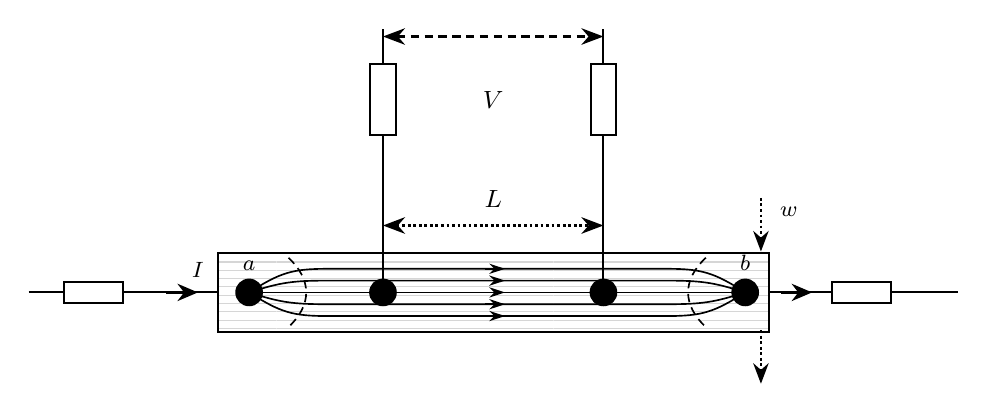
\begin{tikzpicture}[
    every node/.style={font=\small},
    bigdot/.style={circle, fill=black, inner sep=0pt, minimum size=10pt},
    dimline/.style={line width=1.0pt, densely dotted},
  ]

  % ---- sample strip ------------------------------------------------------
  \fill[pattern=horizontal lines, pattern color=black!16] (1.4,-0.5) rectangle (8.4,0.5);
  \draw[wire] (1.4,-0.5) rectangle (8.4,0.5);

  % ---- current leads -----------------------------------------------------
  \draw[wire] (-1.0,0) -- (1.4,0);
  \draw[wire,fill=white] (-0.55,-0.13) rectangle (0.2,0.13);
  \draw[-{Stealth[length=2.6mm,width=2.2mm]},line width=0.8pt] (0.75,0) -- (1.15,0);
  \node[font=\footnotesize,anchor=south] at (1.15,0.06) {$I$};

  \draw[wire] (8.4,0) -- (10.8,0);
  \draw[-{Stealth[length=2.6mm,width=2.2mm]},line width=0.8pt] (8.55,0) -- (8.95,0);
  \draw[wire,fill=white] (9.2,-0.13) rectangle (9.95,0.13);

  % ---- five current-flow lines: uniform in the middle, fanning out
  %      only where they enter and leave the outer contacts ----------------
  \foreach \dy in {0.30,0.15,0,-0.15,-0.30} {
    \draw[line width=0.6pt]
      (1.8,0) .. controls (2.20,{\dy*0.85}) and (2.35,\dy) .. (2.80,\dy)
              -- (7.10,\dy)
              .. controls (7.55,\dy) and (7.70,{\dy*0.85}) .. (8.1,0);
    \draw[-{Stealth[length=2.0mm,width=1.3mm]},line width=0.6pt]
      (4.80,\dy) -- (5.05,\dy);
  }
  % dashed arcs marking where the flow spreads around the current contacts
  \draw[densely dashed,line width=0.6pt]
        (2.30,0.44) .. controls (2.60,0.16) and (2.60,-0.16) .. (2.30,-0.44);
  \draw[densely dashed,line width=0.6pt]
        (7.60,0.44) .. controls (7.30,0.16) and (7.30,-0.16) .. (7.60,-0.44);

  % ---- the four contacts -------------------------------------------------
  \foreach \x in {1.8,3.5,6.3,8.1} { \node[bigdot] at (\x,0) {}; }
  \node[font=\footnotesize,anchor=south] at (1.8,0.16) {$a$};
  \node[font=\footnotesize,anchor=south] at (8.1,0.16) {$b$};

  % ---- voltage leads and the voltmeter -----------------------------------
  \foreach \x in {3.5,6.3} {
    \draw[wire] (\x,0) -- (\x,3.35);
    \draw[wire,fill=white] (\x-0.16,2.00) rectangle (\x+0.16,2.90);
  }
  \draw[densely dashed,line width=0.8pt,
        {Stealth[length=2.8mm]}-{Stealth[length=2.8mm]}] (3.5,3.25) -- (6.3,3.25);
  \node at (4.9,2.45) {$V$};

  % ---- L : distance between the voltage leads ----------------------------
  \draw[dimline,{Stealth[length=2.8mm]}-{Stealth[length=2.8mm]}] (3.5,0.85) -- (6.3,0.85);
  \node[anchor=south] at (4.9,0.95) {$L$};

  % ---- w : sample width --------------------------------------------------
  \draw[dimline,-{Stealth[length=2.6mm]}] (8.3,1.20) -- (8.3,0.52);
  \draw[dimline,-{Stealth[length=2.6mm]}] (8.3,-0.48) -- (8.3,-1.16);
  \node[font=\footnotesize,anchor=west] at (8.42,1.02) {$w$};
\end{tikzpicture}
\end{document}
